%---------------------------------------------------------------------------------------
\chapter{Ideia}

A fim de implementar um sistema que trate dos problemas citados e consiga atingir os objetivos propostos, são necessários processos e a utilização de determinadas tecnologias, citadas no subtópico . 

Os processos principais são três, o cadastramento dos usuários, a automatização do \ac{fpa} e a possibilidade de habilitação de outros processos, por parte dos administradores, com destaque à permutação dos horários já atribuídos e à desativação de um docente em determinada matéria.

\section{Cadastramento dos usuários}

Preliminar à qualquer utilização do \ac{ada}, o Administrador Superior (\gls{superAdmin}), será cadastrado pelos próprios programadores e terá o maior nível de acesso, podendo realizar quaisquer alterações e controlar quais serão os Administradores (\gls{admin}). 

Então, os outros funcionários receberão um link para acessarem o \ac{ada} via Google, pelo e-mail institucional - o que evita acessos não permitidos, e serão atribuídos instantaneamente ao papel de Professor (\gls{professor}); como mencionado, a mudança desse nível de acesso para o de \gls{admin} é realizada pelo \gls{superAdmin}. E acessos posteriores poderão ser através do Google ou do prontuário e senha.

\subsection{Configuração do ambiente}

A configuração do ambiente é um subprocesso, em que o \gls{superAdmin} será responsável por habilitar a possibilidade de \glspl{permuta} e de desativação do docente em uma disciplina; prazos limites à organização; e definição ou atualização dos critérios da atribuição - baseados na legislação vigente e na ordem de prioridade de escolha das disciplinas.

E o \gls{admin} será responsável pela subárea, consequentemente, por subir a grade horária; determinar prazos específicos; autorizar a \gls{permutação} e se deseja participar da aprovação das \glspl{permuta}; controlar os docentes desativados; e adicionar\footnote{Essa adição será manual e de acordo com a prioridade escolhida. Portanto, um subprocesso, onde o \gls{admin} colocará os docentes na ordem e, igualmente, poderá alterá-la em caso de erro ou modificações futuras.} os que participarão de sua subárea. 


\begin{figure}[h]
    \centering
    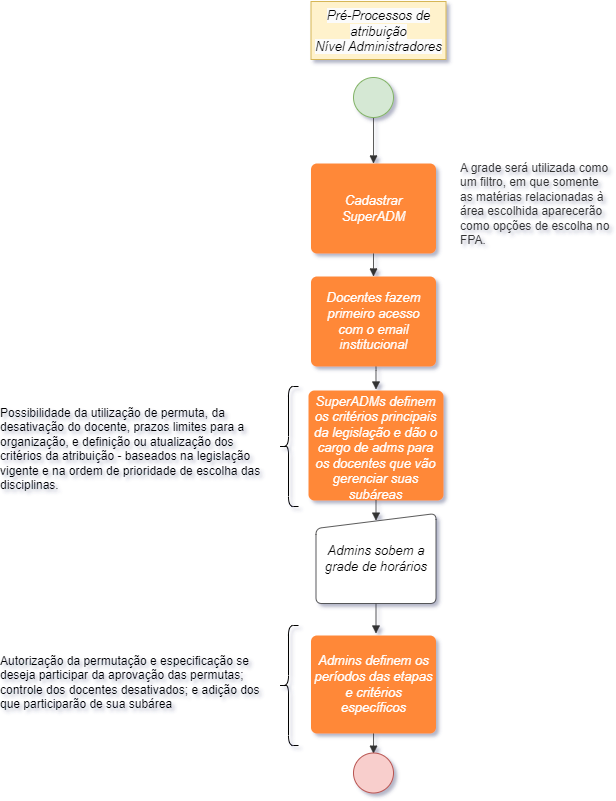
\includegraphics[width=0.85\textwidth]{anexos/Fluxograma/FluxogramaCadastramento.png}
    \caption{Fluxograma dos pré-processos de atribuição}
    \label{fig:figura1} 
\end{figure}

\section{Automatização do FPA}

Finalizada a organização do sistema pelos administradores e todos os docentes cadastrados nas subáreas, eles poderão acessar o sistema e iniciar o processo de escolha da disponibilidade de horários e da preferência de aulas (prioritária e secundária) e de atividades. Conforme é realizado esse processo, o ADA verifica se cada escolha segue os regramentos, e impossibilita a escolha de disciplinas em conflito; igualmente, informa com uma mensagem breve caso o docente selecione uma em que foi desativado. 

\begin{figure}[t]
    \centering
    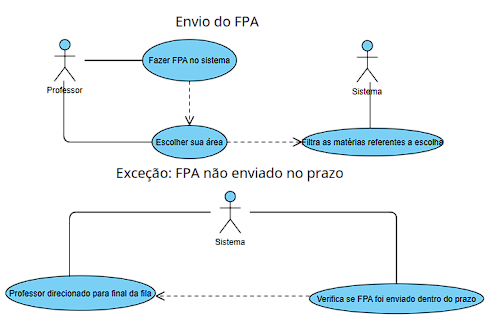
\includegraphics[width=0.7\textwidth]{anexos/CasosDeUso/CasoDeUso_EnvioFPA.png}
    \caption{Caso de uso do envio de preferências}
    \label{fig:figura2} 
\end{figure}

A determinação da preferência de atividades poderá ser modificada dentro do prazo de entrega estabelecido pelo \gls{admin}. Porém, ao encerrar o prazo, o \ac{ada} percorre a lista de docentes, em ordem decrescente, e atribui as aulas de acordo com o selecionado. O processo é interrompido - e é armazenado o que já foi feito - caso haja conflito com uma disciplina já escolhida; assim, aquele docente receberá uma solicitação para alterar sua escolha dentro de determinado prazo.

\begin{figure}[h]
    \centering
    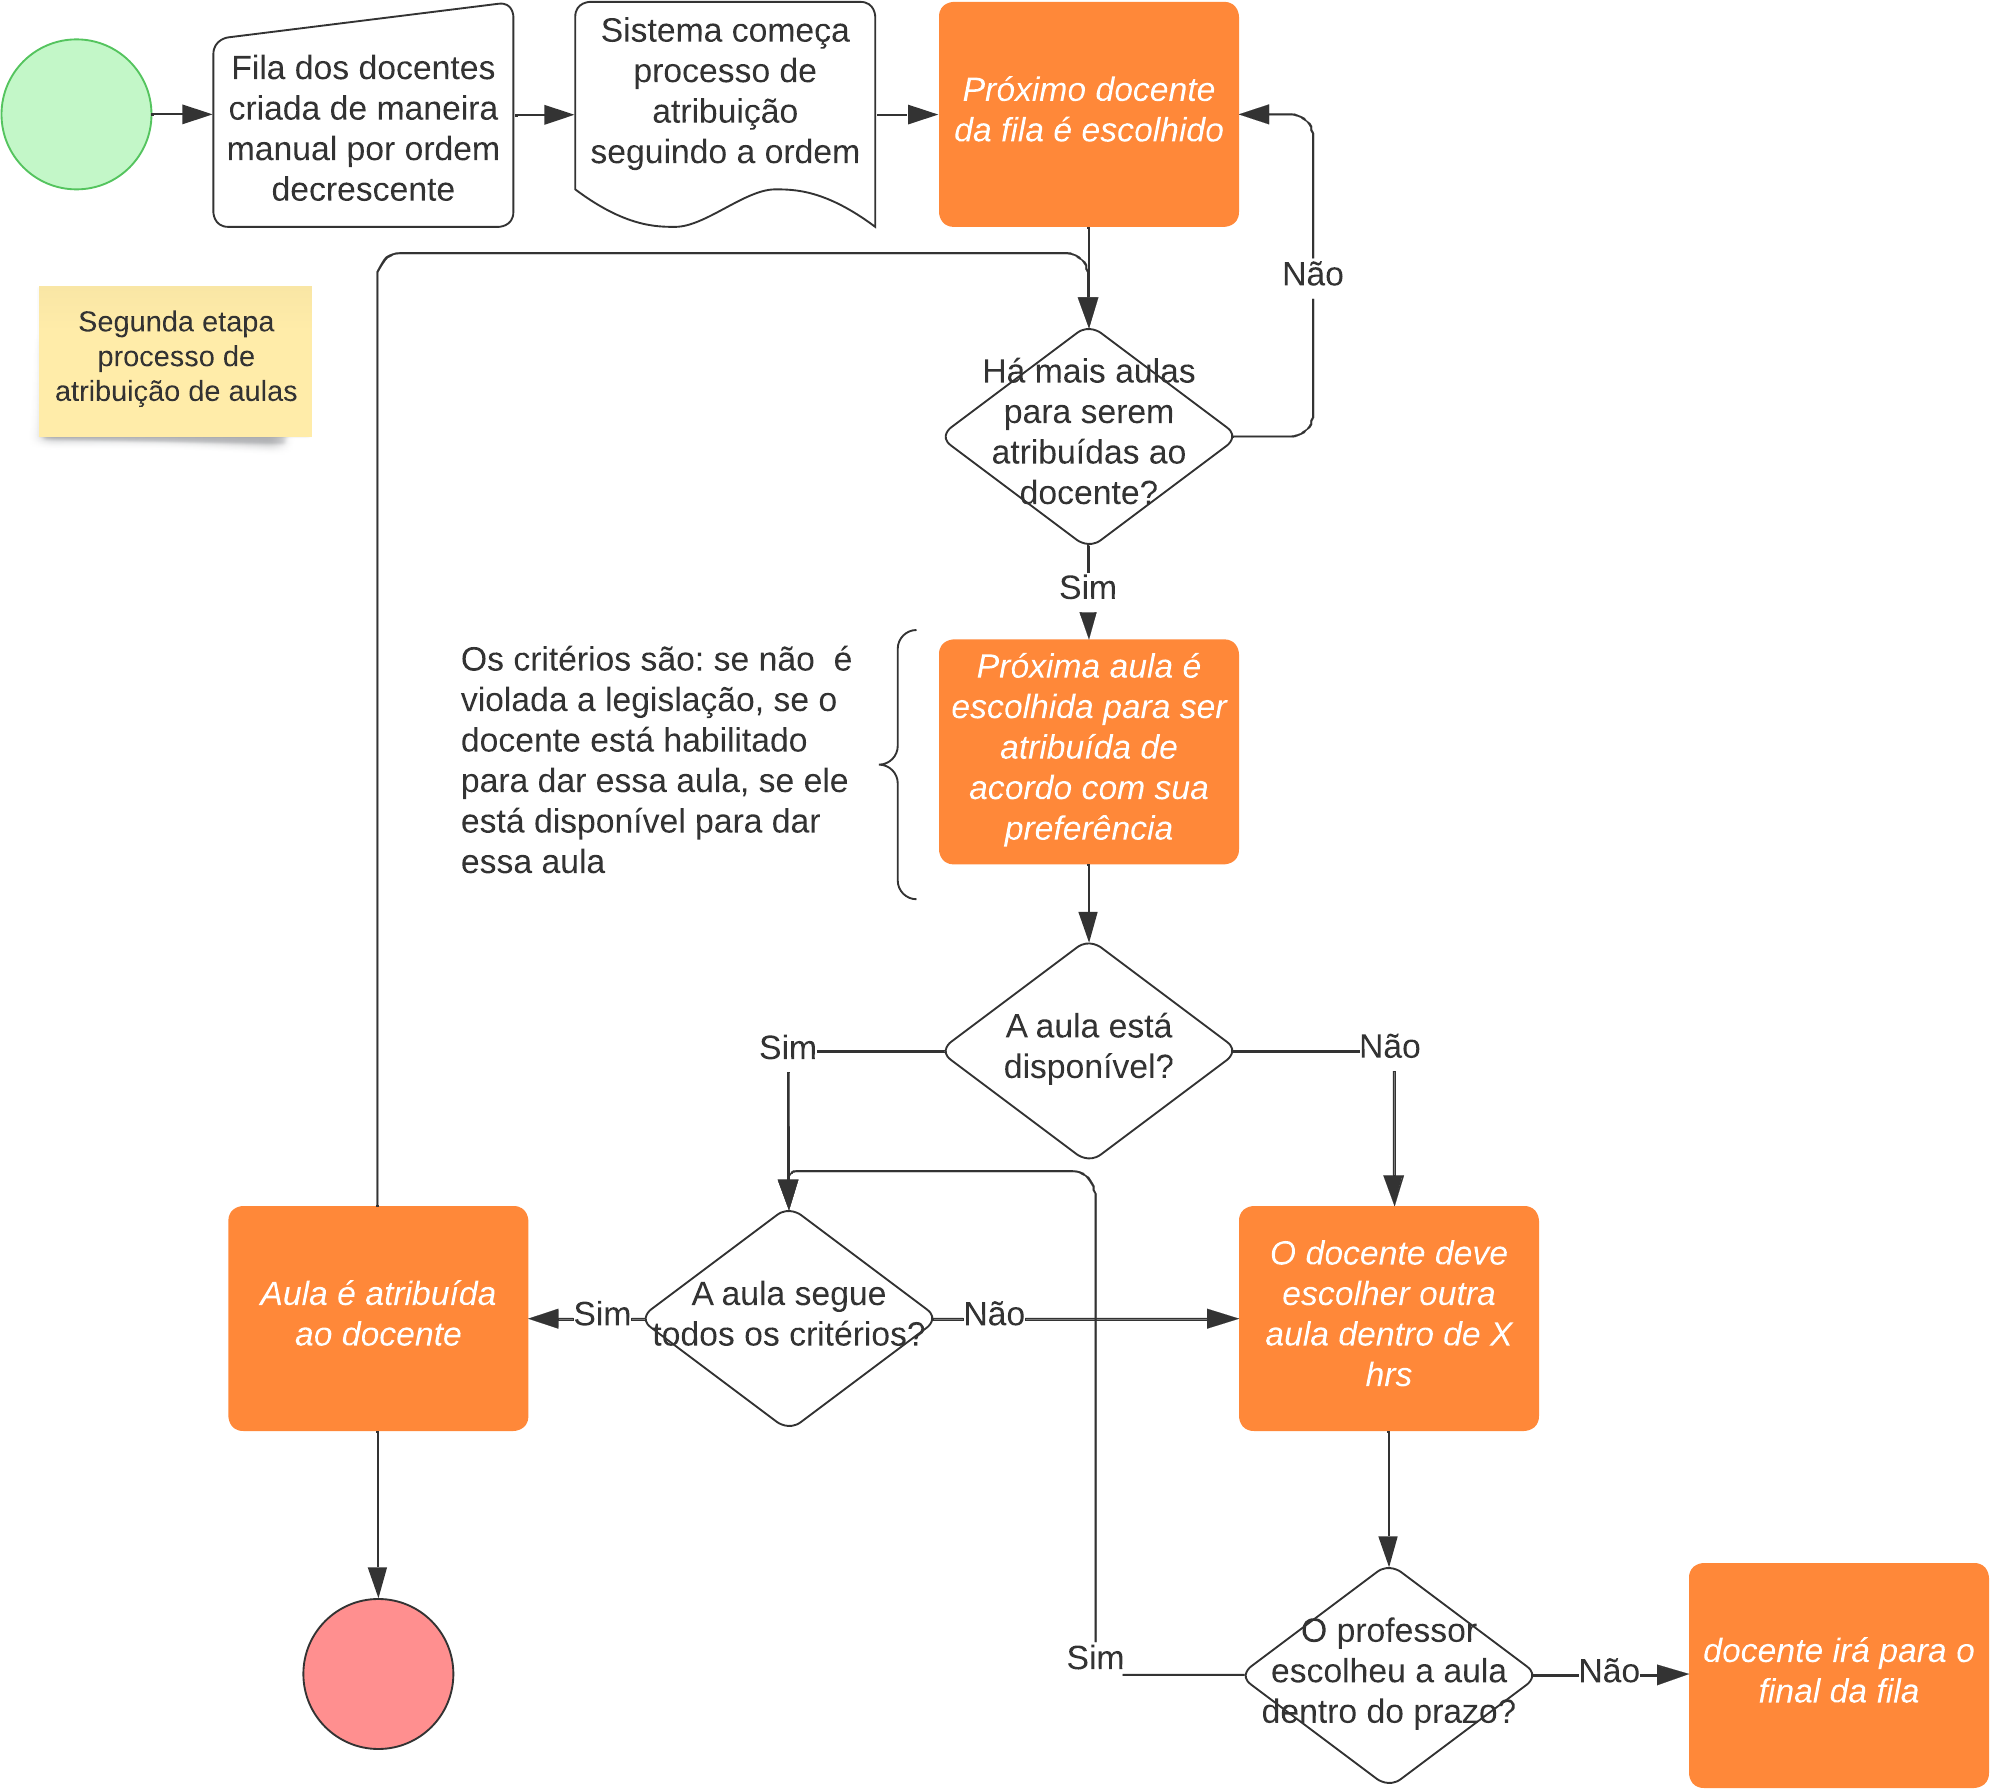
\includegraphics[width=0.7\textwidth]{anexos/Fluxograma/FluxogramaProcessoAtribuicaoAulas.png}
    \caption{Fluxograma da atribuição de aulas}
    \label{fig:figura3}
\end{figure}

\section{Permutação}

A permutação é aberta, caso habilitada com a conclusão da grade pelo sistema. De modo geral, é feita com a solicitação de um docente pela troca de sua aula por uma específica do outro, selecionada na grade. É impossibilitada mais de uma solicitação, ao mesmo tempo, para uma mesma aula; Apenas é liberada quando essa for aceita ou recusada. Igualmente é impossibilidada a solicitação de alguma que descumpra o regramento. 
Caso o \gls{admin} seja moderador, ele terá que aprovar a aceitação da permuta pelo segundo docente.


Por fim, é gerada a grade horária final, onde os docentes e os administradores conseguem visualizar e salvar a atribuição de aulas da subárea. Além da possibilidade de gerar o \ac{fpa} com essa grade pronta.

\begin{figure}[h]
    \centering
    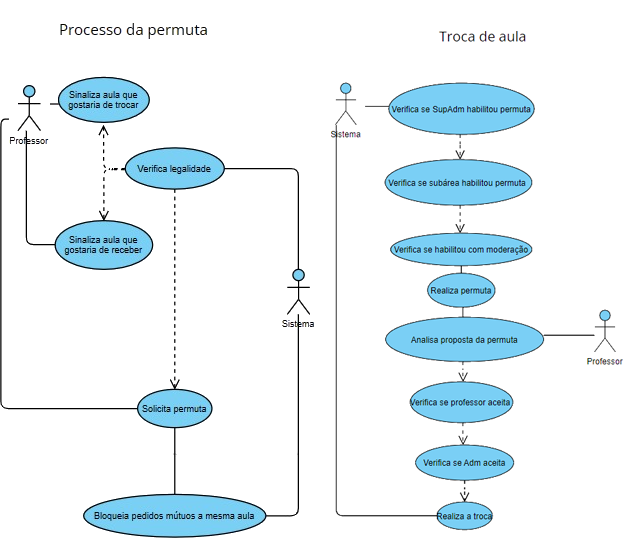
\includegraphics[width=1\textwidth]{anexos/CasosDeUso/CasoDeUso_ProcessoPermutaFULL.png}
    \caption{Caso de uso troca de Aula}
    \label{fig:figura4} 
\end{figure}

\section{Tecnologias e ferramentas aplicadas}

Em vista do desenvolvimento do \ac{ada} de maneira concisa e eficaz, a implementação de tecnologias e suas respectivas ferramentas se faz necessária. Além disso, repositórios de controle de versão e Integrated Development Environment (\ac{ide}) deverão, e serão, utilizados.

\subsection{Tecnologias}
A seguir estão as tecnologias utilizadas, suas características principais e, assim, porque foram escolhidas. A finalidade principal desse conjunto é escrever a aplicação de forma rápida e eficiente, concentrando toda a energia no desenvolvimento e aplicação da lógica, e, logo, poupando tempo em funcionalidades básicas.

\subsubsection{Django}
É um \gls{framework} \textit{web} \textit{\gls{open source}} e de alto nível, desenvolvido em Python, que se baseia no padrão \ac{mtv}, apresentando semelhança com o \ac{mvc}. Assim, segue o princípio \ac{dry}\footnote{Permite que as aplicações sejam desenvolvidas com a maior quantidade de aproveitamento de código possível.}, é moderadamente opinativo \footnote{Flexibilidade que o \gls{framework} dá aos desenvolvedores à resolução dos problemas. Opinativo, já possui uma maneira correta de resolvê-los, sem margens; não-opinativo, não possui essas regras e deixa livre para resolvê-los como quiser. Django equilíbrio entre soluções prontas e arquitetura desacoplada com liberdade na resolução de erros. }e apresenta suporte para erros comuns de segurança. Além desses benefícios, foi escolhido devido a sua aplicação em grandes empresas (como \gls{mozilla} e \gls{pinterest}) e, principalmente, no \ac{suap} do \ac{ifsp}, o que permite manter o padrão de tecnologias no Instituto.
\cite{lucas_2021} \cite{andrade_2019}

\paragraph{\ac{mtv}}
Derivação da arquitetura de software \ac{mvc}, de três camadas, altera a nomenclatura e a relação entre os arquivos. O Model permanece o mesmo, como um canal de conexão entre os tipos de dados e como serão armazenados no Banco de Dados, e a exibição ao ter requisição à View. Essa é responsável, então, pelo gerenciamento das requisições e a lógica de negócio, com a formatação dos dados enviados pelo Model. Por fim, o Template é a interação com o usuário, através de uma exibição estática ou inserção de sintaxe de conteúdo dinâmico, com a renderização dos dados entregues pela View.
\cite{silva_2020}
\
\subsubsection{Python}
É uma linguagem de programação \textit{\gls{open source}} e de alto nível, interpretada em scripts e orientada a objetos, que apresenta tipagem dinâmica\footnote{Tipo do dado é determinado no tempo de execução, de acordo com o valor do dado, não a partir da sua variável.} forte. Logo, prioriza a agilidade por meio de sua fácil compreensão, sintaxe menor e simplificada, sem muitas exigências gramaticais. E é por isso que foi escolhida, uma ótima opção que supriu de forma excelente a necessidade de uma aprendizagem rápida e fácil codificação nos dispositivos do \ac{ifsp}, além de poder ser facilmente integrada a outras linguagens de programação populares, caso seja necessário no decorrer do projeto.
\cite{amazon_2023} \cite{melo_2021}

\subsubsection{AJAX}
O \ac{ajax} é uma técnica de desenvolvimento \textit{web}, caracterizada pela criação de aplicações interativas através de requisições ao servidor. Uma junção das funcionalidades do \ac{js} com a troca dos dados, armazenados e transmitidos, nesse caso, pelo \ac{json} (mais próximo do \ac{js}). Foi escolhido justamente por servir como um canal de comunicação independente entre o cliente e o servidor.
\cite{andrei_2019} \cite{carvalho_2007}

\subsubsection{JavaScript}
É uma linguagem de programação de alto nível e interpretada em scripts, com recursos de \ac{oo} e \ac{api}, que apresenta tipagem dinâmica. Assim, por meio de um funcionamento assíncrono \footnote{A programação assíncrona é uma técnica na qual o programa inicia uma tarefa e ainda é capaz de executar simultaneamente outros eventos, ao invés de bloquear processos para esperar o término da execução.}, usa trechos dos códigos HTML para renderizar funções que proporcionem uma interação dinâmica local com o conteúdo da página. Foi escolhida para, em conjunto com o \ac{ajax}, proporcionar essa dinamicidade em tempo real, recarregamento automático.
\cite{mozilla_2023} \cite{melo_2021}

\subsubsection{HTML}
O \ac{html} é uma estrutura responsável pela exibição dos dados no navegador \textit{web}, caracterizado por seus elementos hierarquizados e sua marcação que abriga elementos como tags. Na aplicação ADA, é utilizada nos templates, explicados no parágrafo 2.4.1.1.1 .
\cite{mozilla_2023b}

\subsubsection{CSS}
O \ac{css} é uma linguagem de marcação, responsável pela estilização de elementos \ac{html}. Foi escolhido a fim de ajudar na formatação dos templates em detalhes específicos que, por vezes, não são compreendidos pelo framework, pois esse é mais genérico.
\cite{totvs_2020}

\subsubsection{Bootstrap}
É um \gls{framework} \textit{front-end}, logo, voltado à estilização, e \textit{\gls{open source}}. Foi escolhido devido à agilidade no desenvolvimento da página para o usuário, característica pelos frameworks, e, principalmente, devido à responsividade proporcionada.
\cite{andrei_2019} \cite{lima_2021}

\subsubsection{SQLite3}
\ac{sgbd}, o SQLite é uma biblioteca em linguagem C, \textit{\gls{open source}}, acoplada ao banco de dados \ac{sql}. Escolhido porque entrega o banco em conjunto com a aplicação (é embutido), sem a necessidade de um servidor, já que optamos por realizar a arquitetura \ac{mtv} em vez de Cliente/Servidor.
\cite{silva_2007} \cite{carlos_2019}

 \subsection{Hospedagem}
 A fim de ter uma instância em nuvem e conseguir fazer a hospedagem do site, foi utilizada a \ac{aws}. É uma plataforma que disponibiliza diversos serviços de computação em uma rede de servidores remotos. Assim, é possível criar instâncias de máquinas com sistema operacional Windows ou Linux, de modo que a aplicação funcione constantemente, sem necessitar que um computador pessoal fique ligado. 

 Somente com ela já é disponibilizada a aplicação na \textit{web}. Todavia, o acesso é difícil, pois aparecerá somente o endereço IPv4 público da máquina virtual criada. Para resolvê-lo, foi comprado o domínio \url{https://mottarios.cloud/} no \textit{website} Hostinger.

 \subsection{Criptografia}
A criptografia, para fornecer uma aplicação segura, foi configurada seguindo o protocolo \ac{https}, 

De forma a verificar seu devido funcionamento, foi utilizada a certificadora \textit{Let’s Encrypt}. Assim, teve uma confirmação de que há controle sobre o domínio citado anteriormente, e, com isso, foi gerado um certificado \ac{ssl}/\ac{tls} para ele. Após adicionar o certificado, a aplicação atingiu nota A no \textit{SSL Labs}. Para mais informações: \url{https://www.ssllabs.com/ssltest/analyze.html?d=mottarios.cloud}
\
\begin{figure}[h]
    \centering
    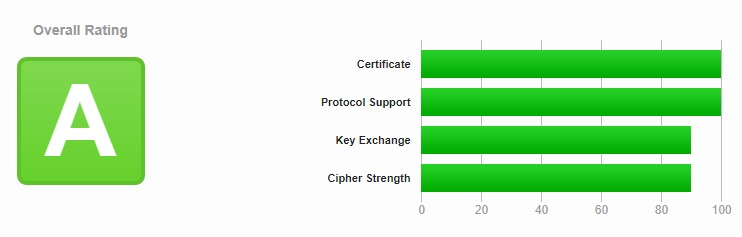
\includegraphics[width=1.00\textwidth]{anexos/DiagramaDeArquitetura/Certificado_NotaA.jpeg}
    \caption{Certificado SSL/TLS}
    \label{fig:figura1} 
\end{figure}

\subsection{Ferramentas}

\subsubsection{Controle de Versão}
É utilizado o \ac{svn}, uma ferramenta que armazena projetos e todas suas versões em um servidor centralizado. Escolhido devido à padronização dos projetos e devido à capacidade de armazená-los de forma segura. Igualmente, é utilizado o \gls{github}, de forma secundária, devido à familiaridade e à melhor organização, principalmente tratando-se do uso de \textit{branchs}.

\subsubsection{Documentação}
É utilizado o Overleaf, um editor e compilador \textit{online} de \gls{latex}. A fim de seguir a padronização dos projetos anteriores e para uma produção mais dinâmica dos documentos \gls{latex}, já que permite o compartilhamento dos arquivos entre outras pessoas e a edição simultânea. 

\subsubsection{Programação}
É utilizado o \ac{vscode}, um editor de código-fonte criado pela Microsoft. Foi escolhido devido a sua dinamicidade para codificação e a familiaridade que os membros da equipe já possuem com a ferramenta. 

Ademais, também é utilizado o codespace, que, por sua vez, é um ambiente de desenvolvimento hospedado em nuvem, promovido pela plataforma GitHub. Assim, é possível programar através do navegador, sem precisar de uma aplicação instalada na máquina, facilitando a programação no \ac{ifsp}. 

\subsection{Diagrama de Arquitetura}

\begin{figure}[h]
    \centering
    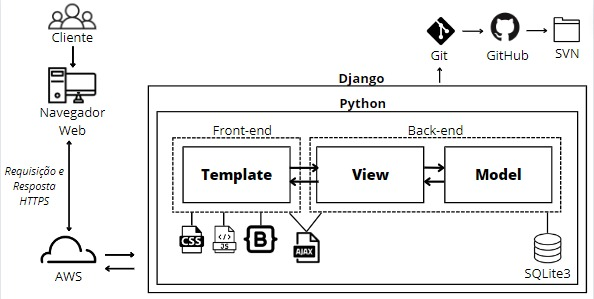
\includegraphics[width=0.96\textwidth]{anexos/DiagramaDeArquitetura/DiagramaDeArquitetura.jpeg}
    \caption{Diagrama de arquitetura}
    \label{fig:figura1} 
\end{figure}

%  LISTA
% \begin{itemize}
%   \item List entries start with the \verb|\item| command.
% \end{itemize}

%---------------------------------------------------------------------------------------





